% Simple tree diagram using the Tikz library.

\documentclass{article}
\usepackage{tikz}
\usepackage[left=2cm,right=2cm,top=2cm,bottom=2cm]{geometry}

\usetikzlibrary{trees}

\title{Tikz Library}
\author{Soorya Kumar}
\date{\today}

\begin{document}
	\maketitle
	
	\section*{Question}
		{\large Develop a LaTeX script to design a simple tree diagram or hierarchical structure in the document with appropriate labels using the Tikz library.\\}
		
	\section*{Tree Diagram}
		\begin{center}
			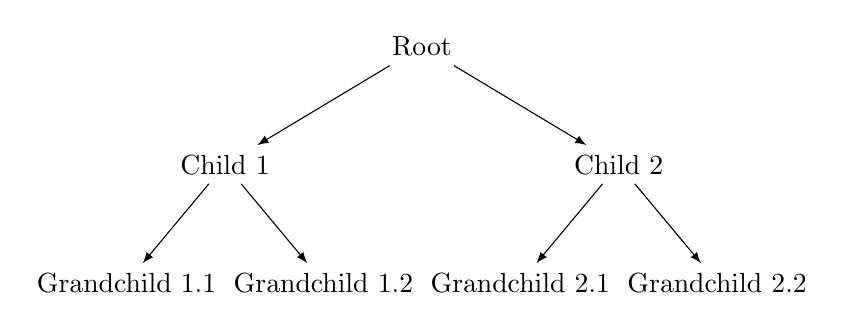
\begin{tikzpicture}[
				level 1/.style={sibling distance=50mm},
				level 2/.style={sibling distance=25mm},
				edge from parent/.style={->,draw},
				>=latex]
				
				% Root node
				\node {Root}
				child { node {Child 1}
					child { node {Grandchild 1.1} }
					child { node {Grandchild 1.2} }
				}
				child { node {Child 2}
					child { node {Grandchild 2.1} }
					child { node {Grandchild 2.2} }
				};
			\end{tikzpicture}
		\end{center}
	
\end{document}
